\begin{frame}{Ice People Family Tree}
    \note{
        Diving into the narrative intricacies of the 47-book saga,
        we're brought face-to-face with a sprawling family tree that traces its lineage
        back to the matriarch Silja Arngrímsdóttir and her cursed beau, Þengill the good.

        Their descendants' tangled relationships are laid out here,
        and it's impossible to ignore the density of the connections --
        hinting at a significant amount of inbreeding.
        This compact lineage, while perhaps challenging for readers (and narrators!)
        to digest given its incestuous undertones, does offer us a silver lining --
        it's surprisingly \emph{slide-friendly}. Managing to represent 17 generations in one visual
        would generally be a challenge, but the Ice People's family tree is a rare exception.

        On the topic of the curse, those afflicted by it have been highlighted with solid colors.
        The color codes represent their nature: yellow for the \emph{virtuous},
        green for the \emph{malevolent}, and pink for those who found \emph{redemption},
        transitioning from darkness to light.

        As we scan through the tree, it's curious to note that the distribution of the curse
        doesn't seem to follow a strict genetic pattern. Entire generations sometimes escape its grasp,
        suggesting that Margit perhaps allowed a degree of creative freedom over genetic accuracy in
        deciding who bears the curse.

    This intricate web of relationships, filled with cursed figures,
        highlights the need for a data-driven approach to unravel and understand Margit's artistic choices.
}
    \centering
    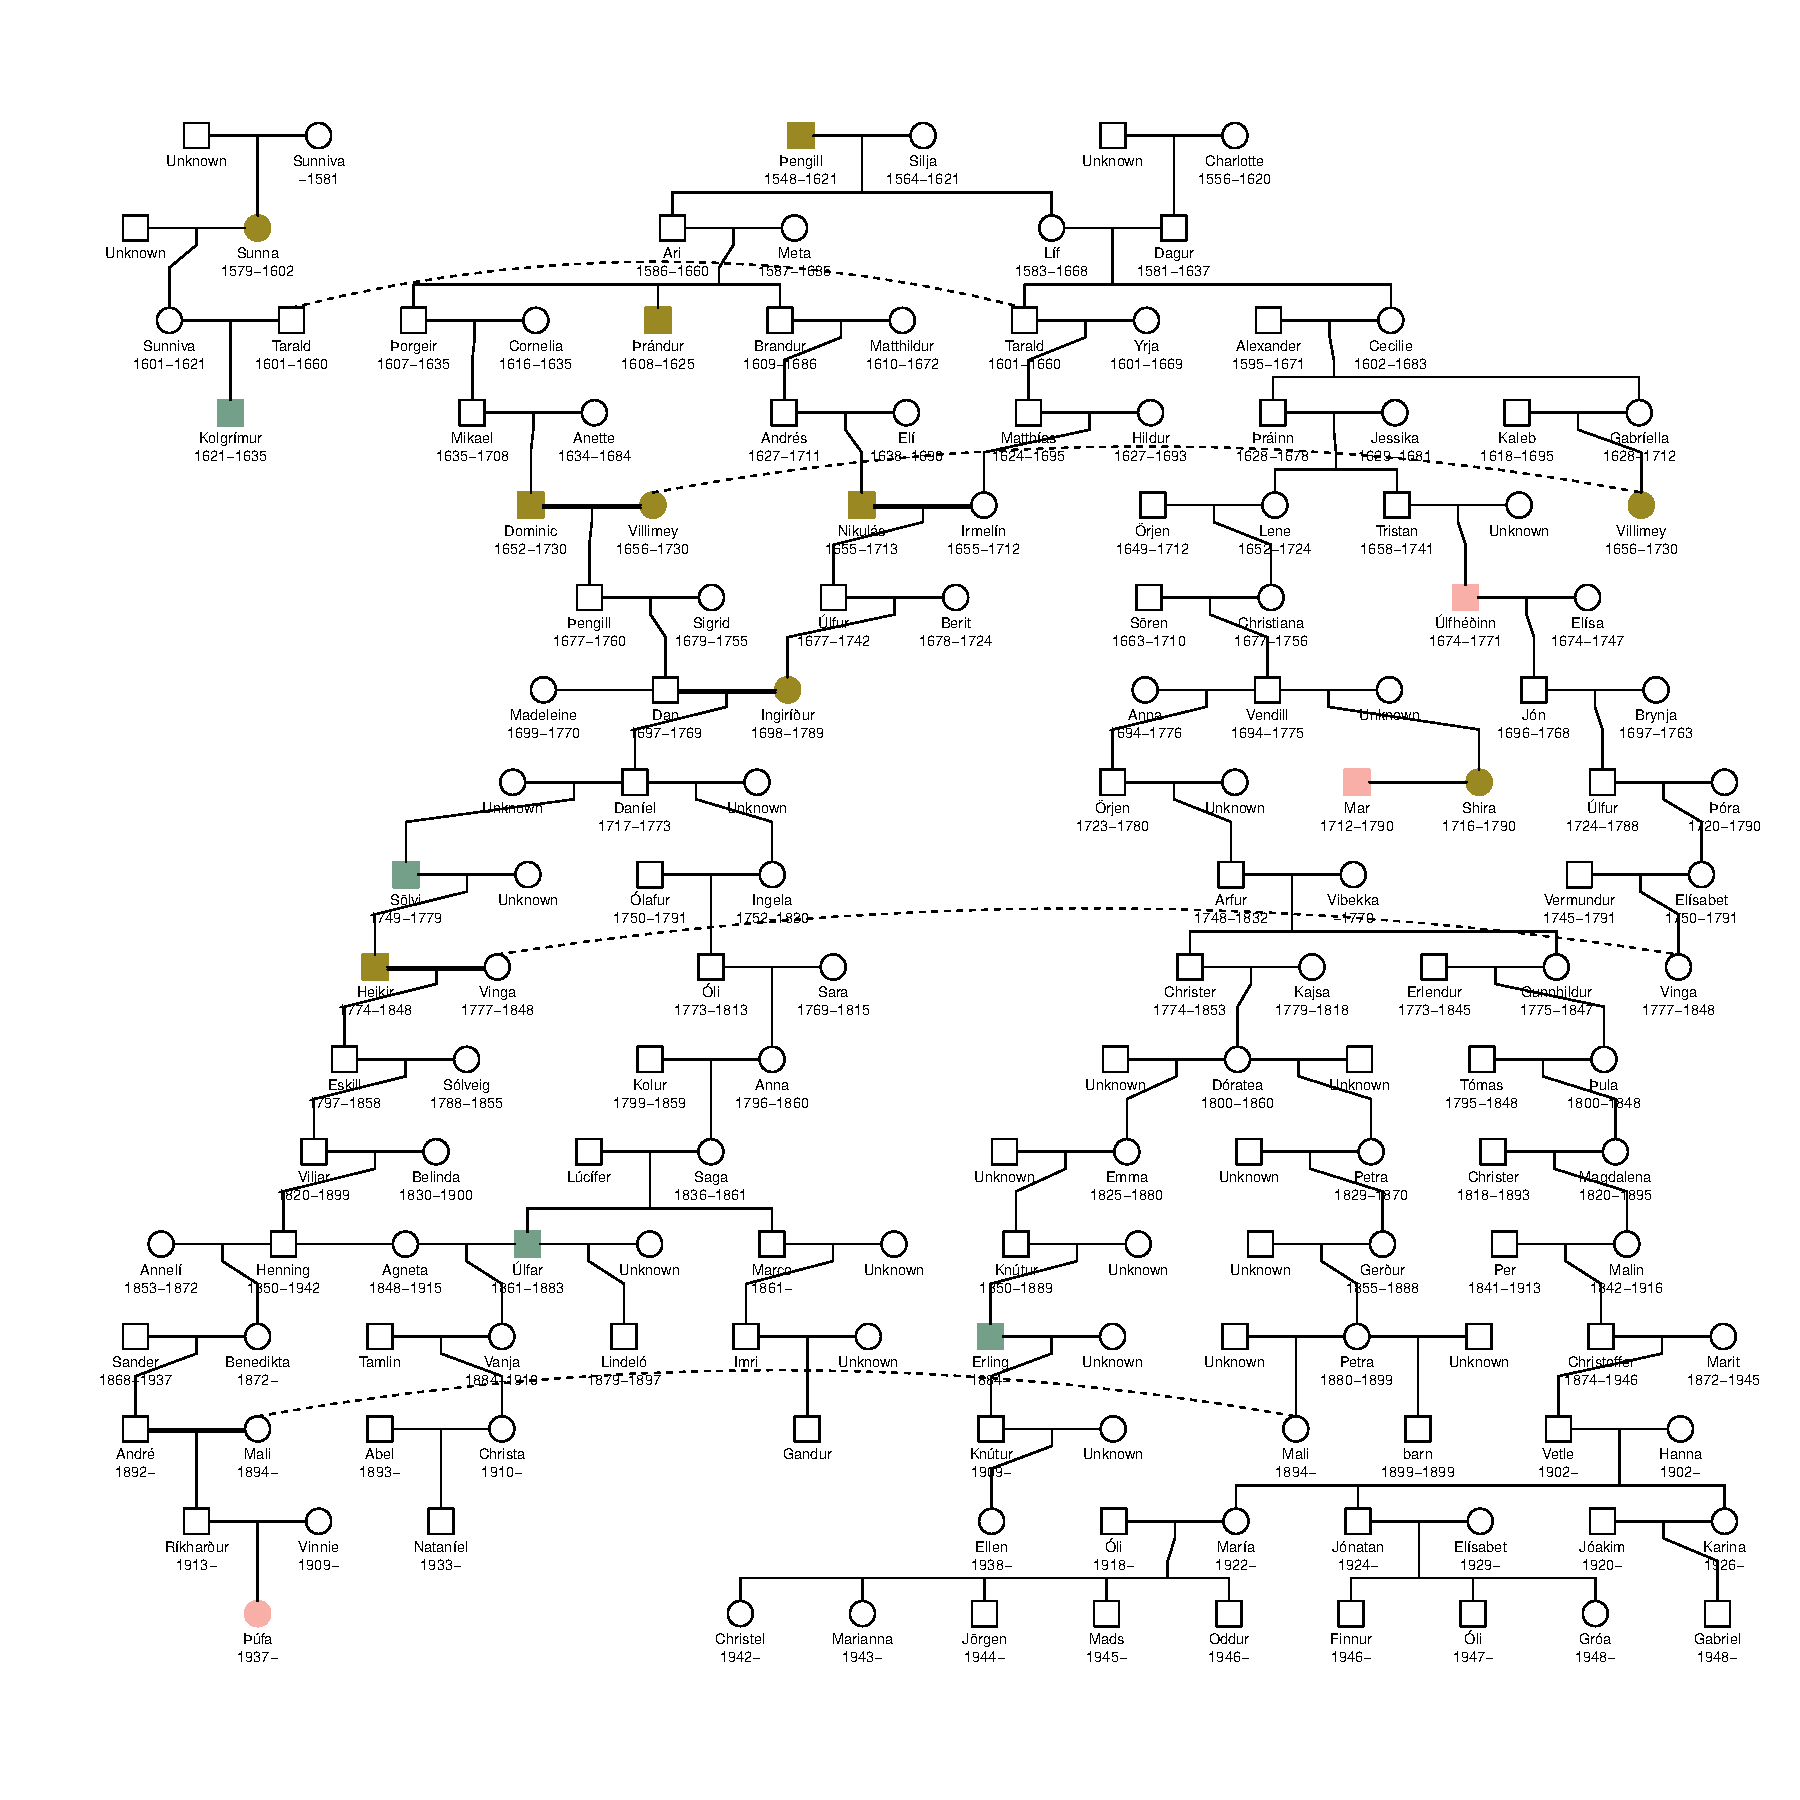
\includegraphics[height=.9\textheight]{../rek-data-beers/R/figures/family_tree}
\end{frame}

\begin{frame}{Ice People Family Gantt Chart}
    \note{
    To decipher the complex family tree and its concurrent relationships,
        we turned to a \emph{data transformation}: the \emph{Gantt} chart,
        usually a tool for project timelines, but here, it's a brilliant
        visualization of lifespans and intersecting narratives.

    As we traverse this visual representation, you'll notice each individual's
        lifespan is represented by a horizontal bar.
        Births commence on the left and deaths conclude on the right.
        Our familiar color-coding prevails: yellow signifies the benevolent,
        green the malevolent, and pink the redeemed.

    Spanning from the mid-1600s to the 1960s, this chart offers clear insights
        into overlapping lifetimes, painting a vivid picture of contemporaneous
        characters.

    A pattern quickly emerges: Margit frequently intertwines character narratives,
        often through romantic unions. This attraction amongst the Ice People is
        both a narrative device and a manifestation of their shared, cursed lineage.
        While generations pass, the family typically hovers around 20 living members,
        swelling to 30 towards the end.

    Worth noting is the general pattern of having 1-2 cursed individuals alive at
        any point. Yet, in the early 1700s, a deviation occurs with six concurrent
        cursed beings. And while Mar doesn't emerge until later in the narrative,
        he isn't directly from the Ice People lineage but descends from the Taranqyes.
        This clan shares a common ancestor with the Ice People, tracing back to
        the malevolent Þengill the Bad.
    }
    \centering
    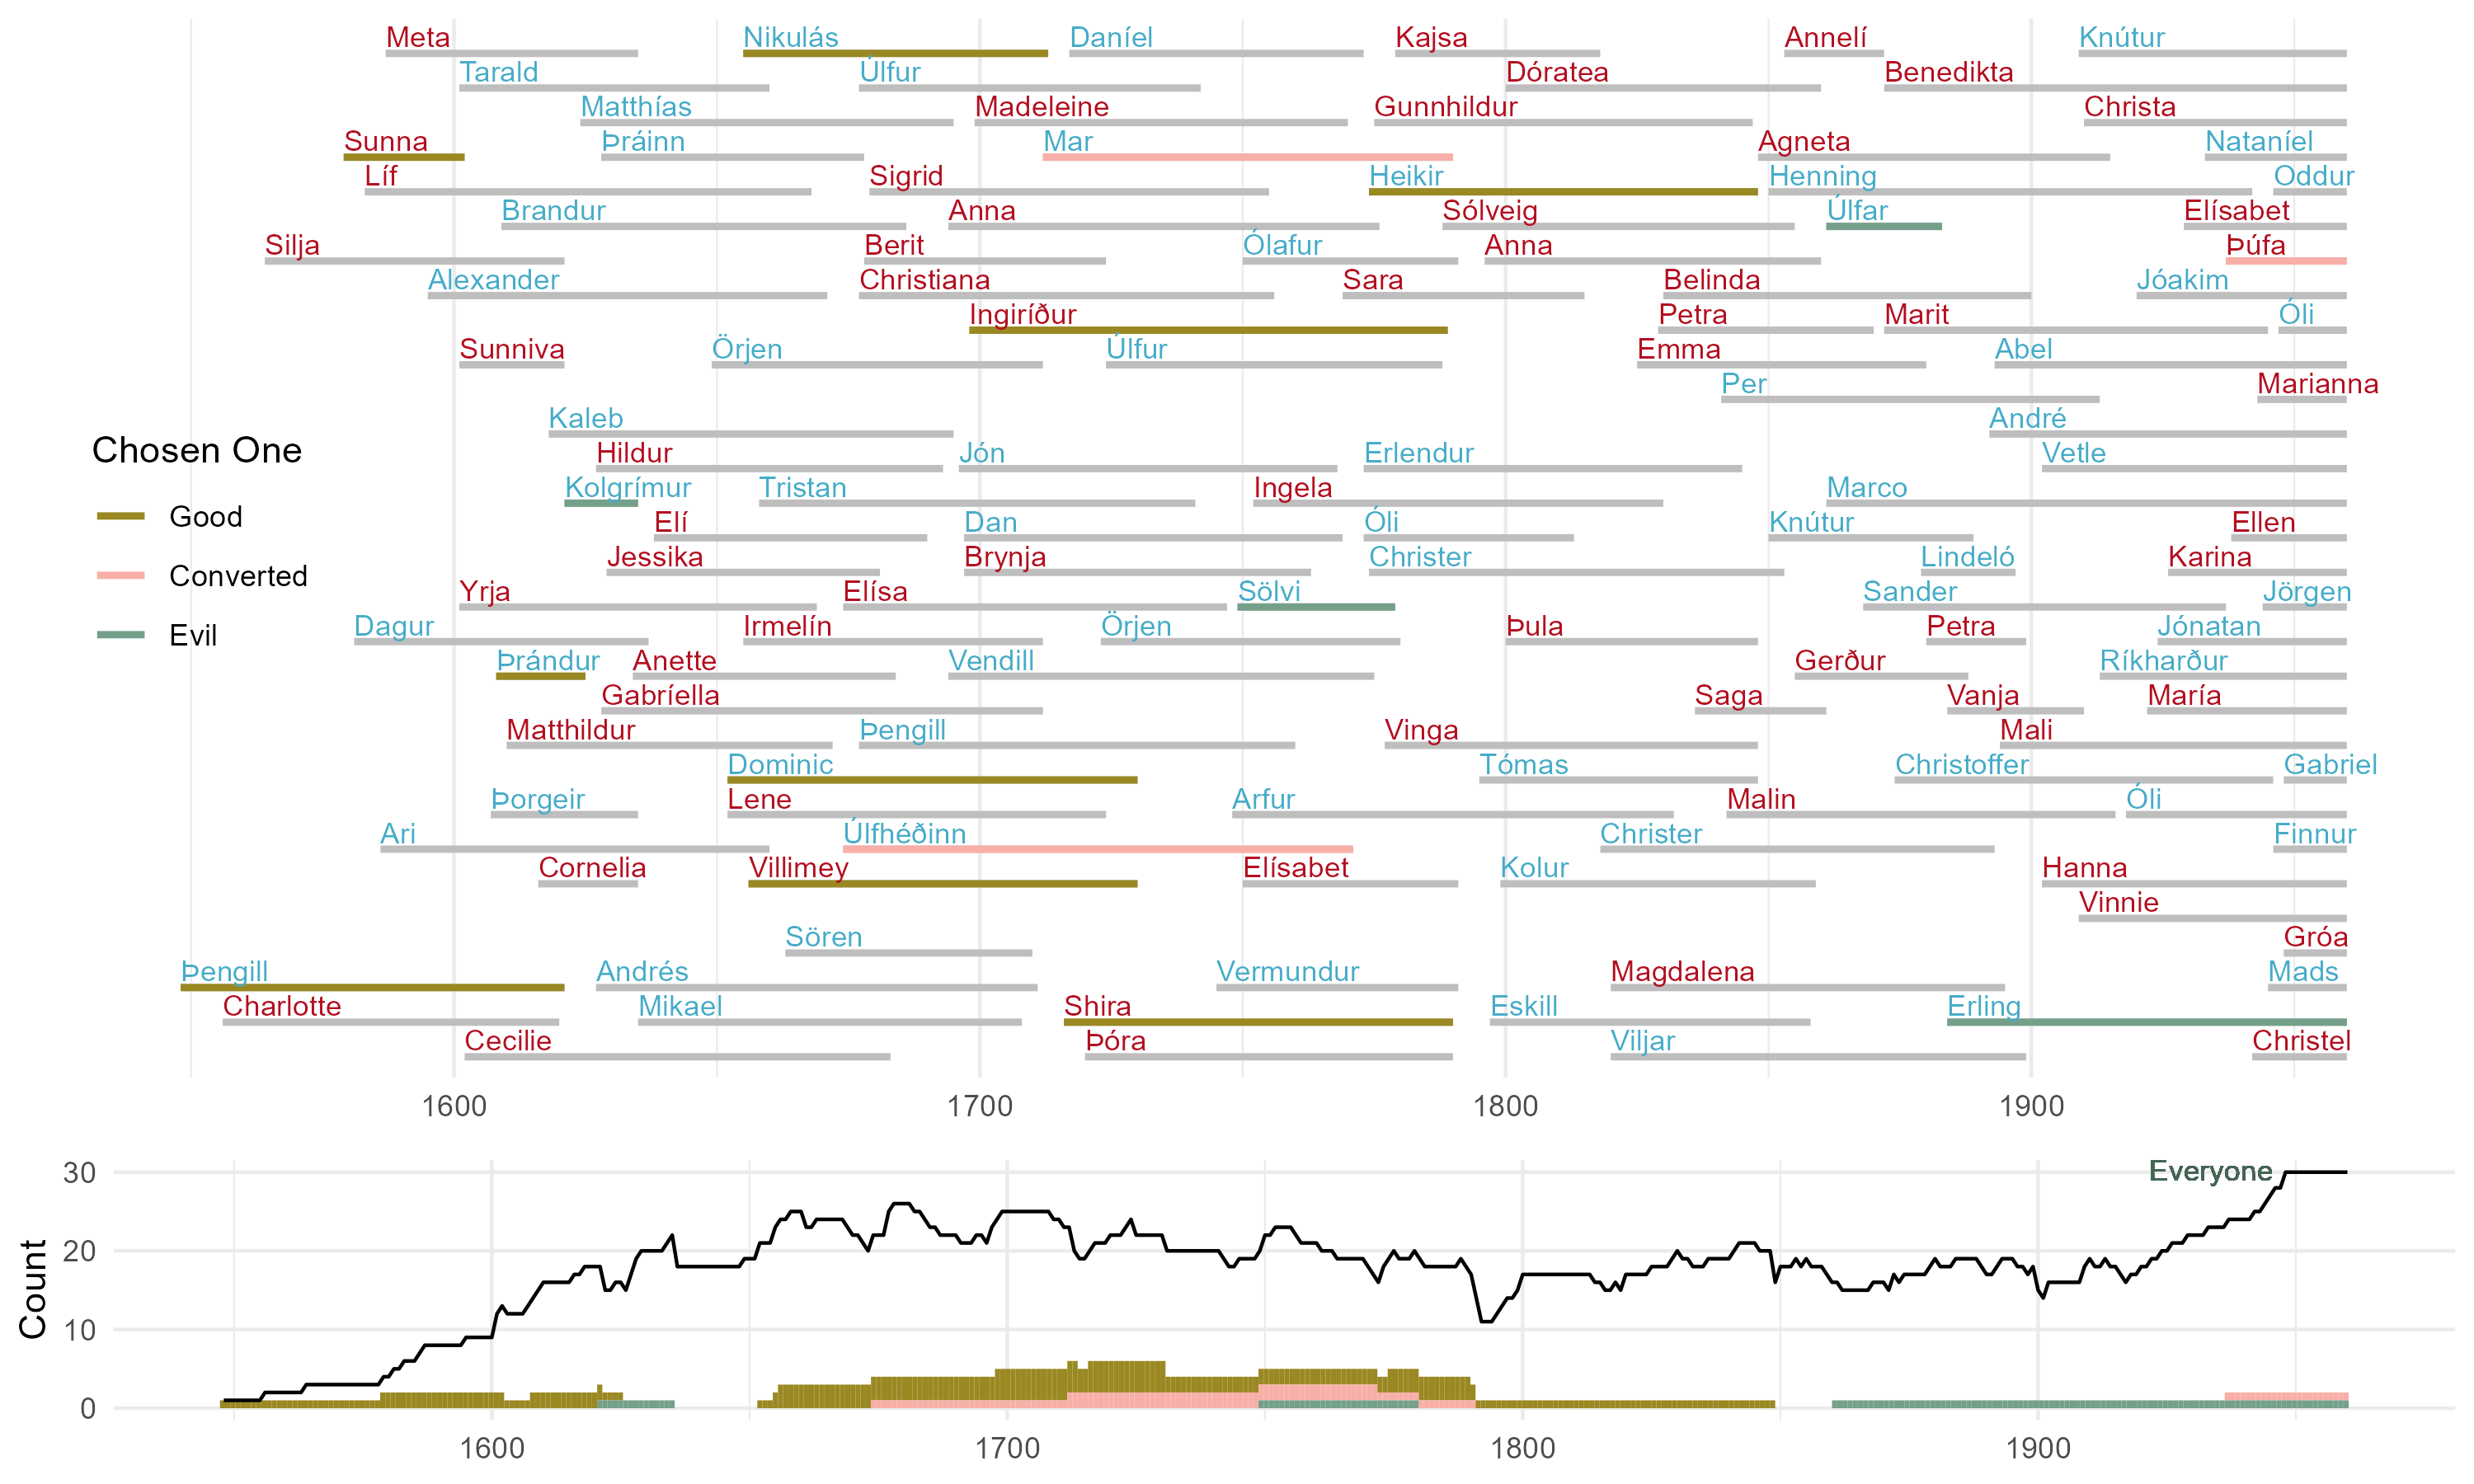
\includegraphics[width=\textwidth]{../rek-data-beers/R/figures/family_gantt}
\end{frame}

\begin{frame}{Lifespan of the Ice People}
    \note{In the Ice People saga, women tend to live shorter lives than men,
        a deviation from our real-world trends where women typically outlive men.

        Sandemo provides reasons: childbirth is particularly perilous for women
        birthing cursed children with challenging triangular shoulders.
        However, those who survive childbirth often lead long lives.

        This risk-loving behavior is especially pronounced in cursed males,
        whose malevolence and recklessness often lead to dramatic but brief lives.
    }
    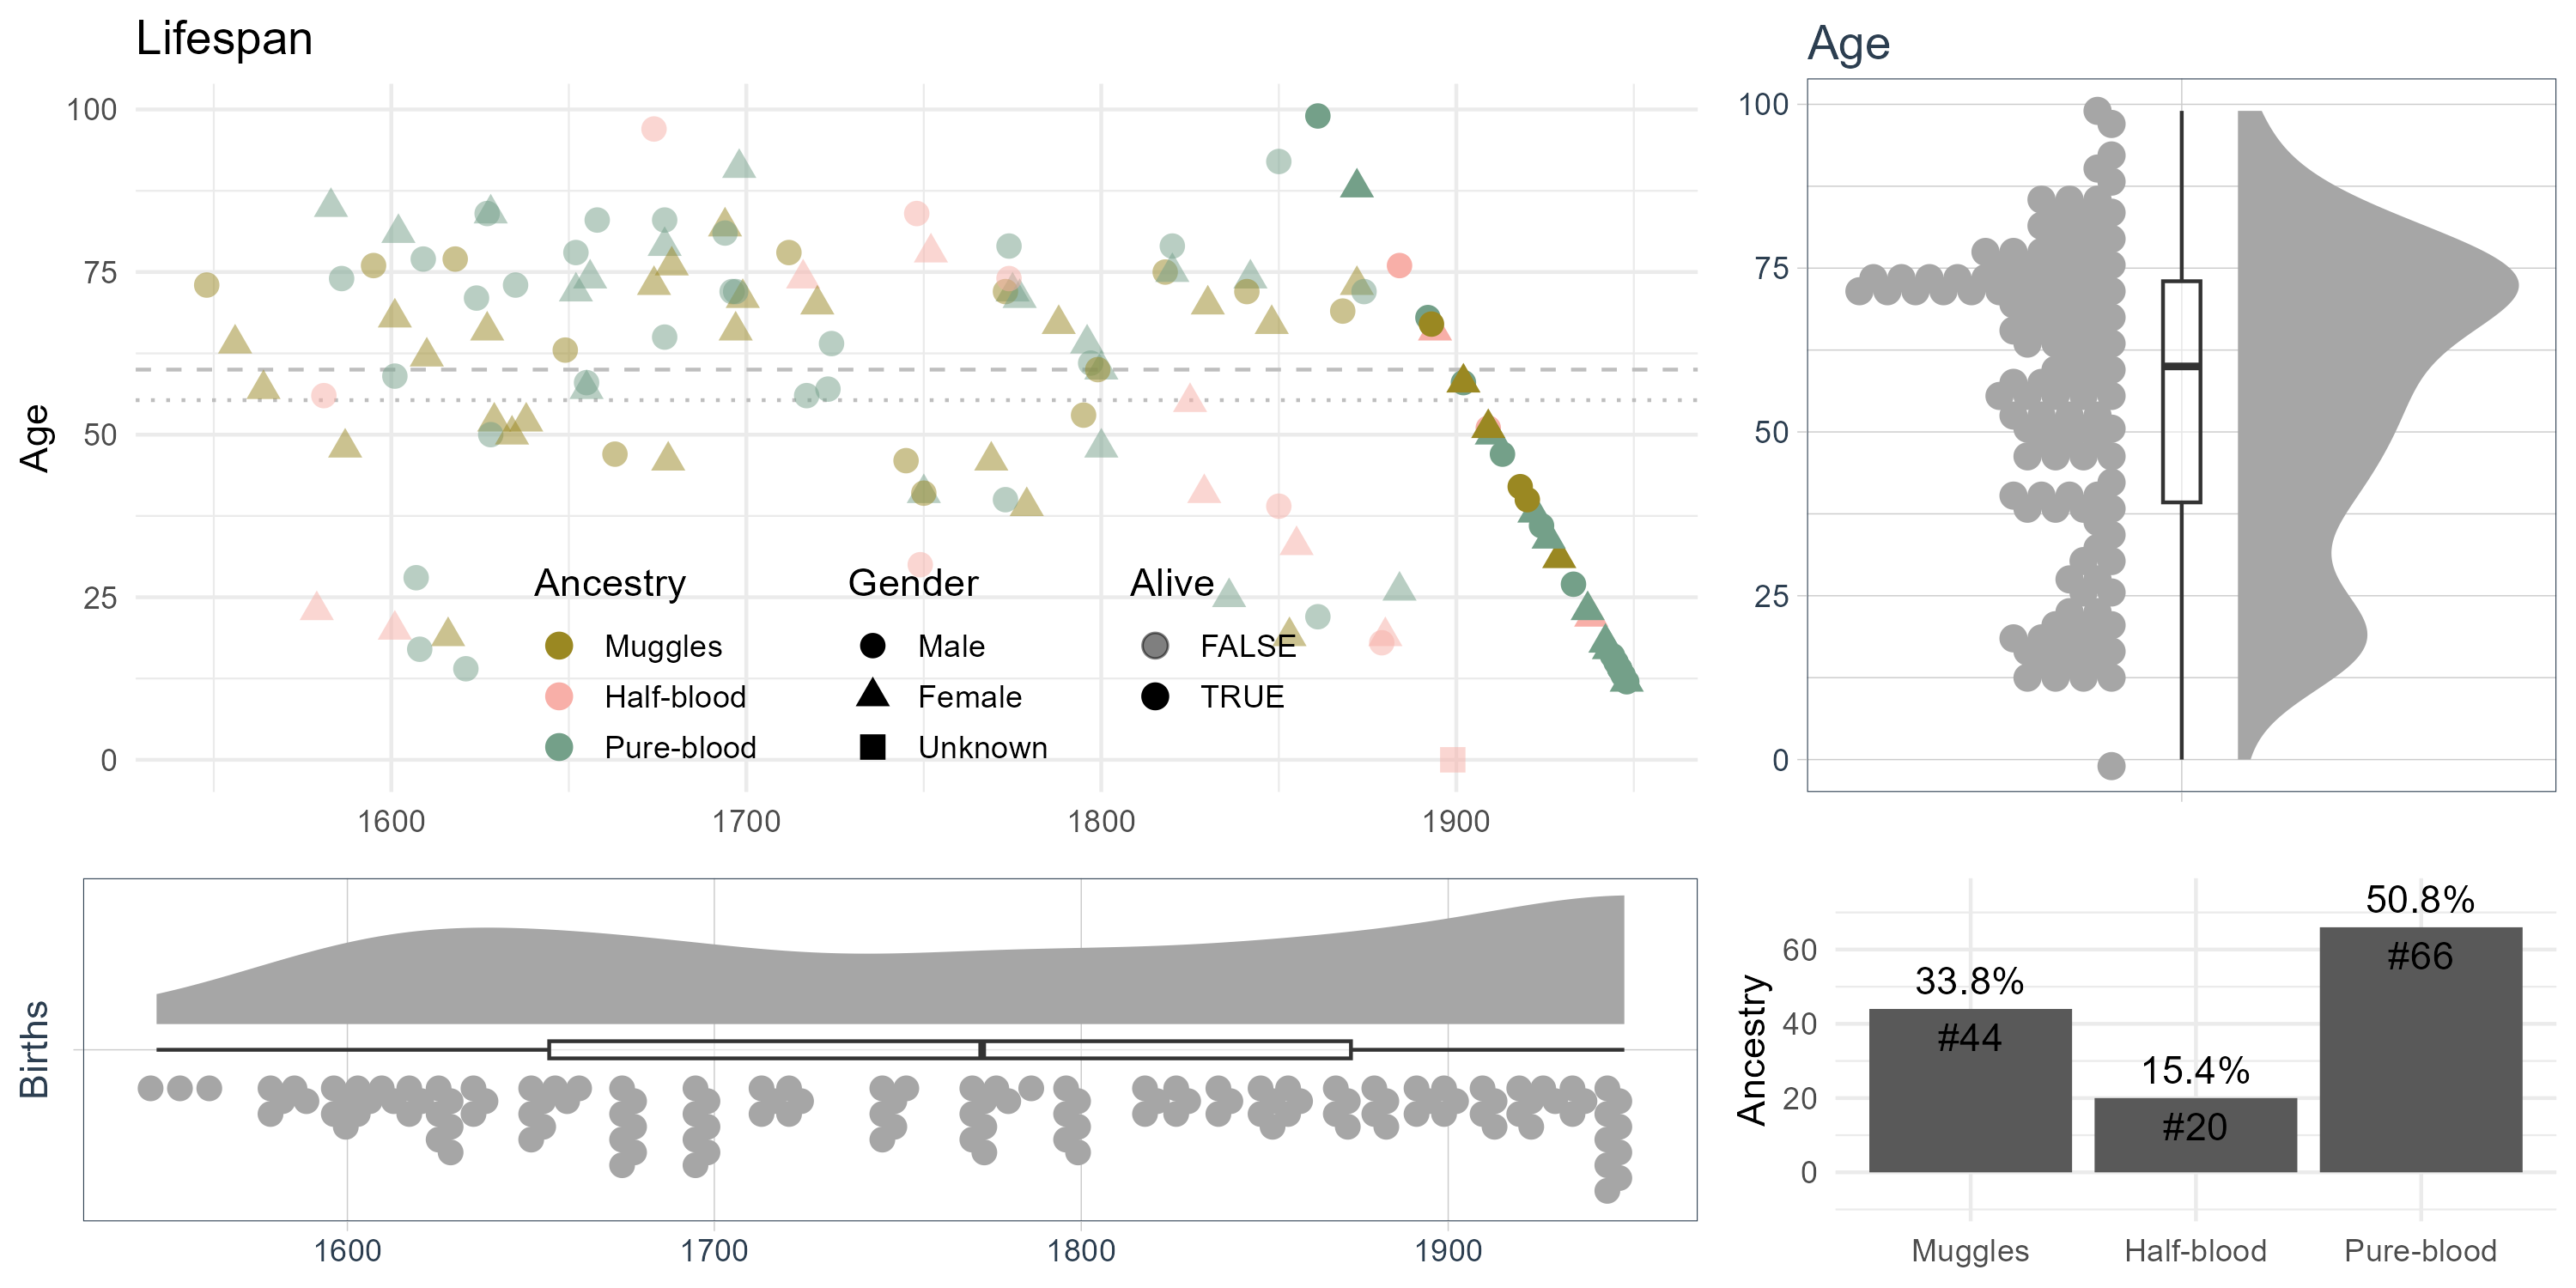
\includegraphics[width=\textwidth]{../rek-data-beers/R/figures/family_birth}
    \vspace{-18pt}
    \begin{itemize}
        \item Average woman lives 58.5 years (median 65, $n=50$)
        \item Average man lives 62.5 years (median 71, $n=49$)
        \item 1 centenarian, 4 people live to 90, 14 live to 80, 46 live to 70
    \end{itemize}
\end{frame}

\begin{frame}{Parental Birth Age \& Spousal Age Gap}
    \note{Diving deeper into the Ice People saga, several distinct patterns emerge that deviate from real-world norms. Women in the narrative, acutely aware of the peril that birthing a cursed child poses, often opt to delay motherhood. Their caution is rooted in the chilling potentiality: the child’s triangular shoulders, a telltale sign of the curse, which can lead to fatal complications during childbirth.

Yet, another stark reality in this saga is the number of children growing up without a pivotal parental figure. Out of 66 children born, 22 are left navigating life without either a mother or a father. This isn't a result of divine intervention, but rather the cold abandonment by parents. Especially those outside the Ice People lineage can find themselves overwhelmed by the possibility of raising a potentially cursed child.

However, when women do decide to have children, their family size varies widely. If one child turns out not to be cursed, there's a hesitancy to expand the family further, haunted by the looming fear that the next might not be so fortunate. Yet, in situations where a cursed member already exists in a generation, the shackles of dread seem to fall away, leading to larger families. The logic here, though puzzling by real-world standards, is that the generation's "curse quota" is already filled, so they might as well have more kids.

Amidst these unique nuances, one element remains conventional: the age dynamics between couples. Echoing real-world tendencies, 85\% of Ice People marriages feature an older husband, with an average age gap of around three years. Beyond this touch of tradition, the world of the Ice People oscillates between the realms of the ordinary and the extraordinary.
}
    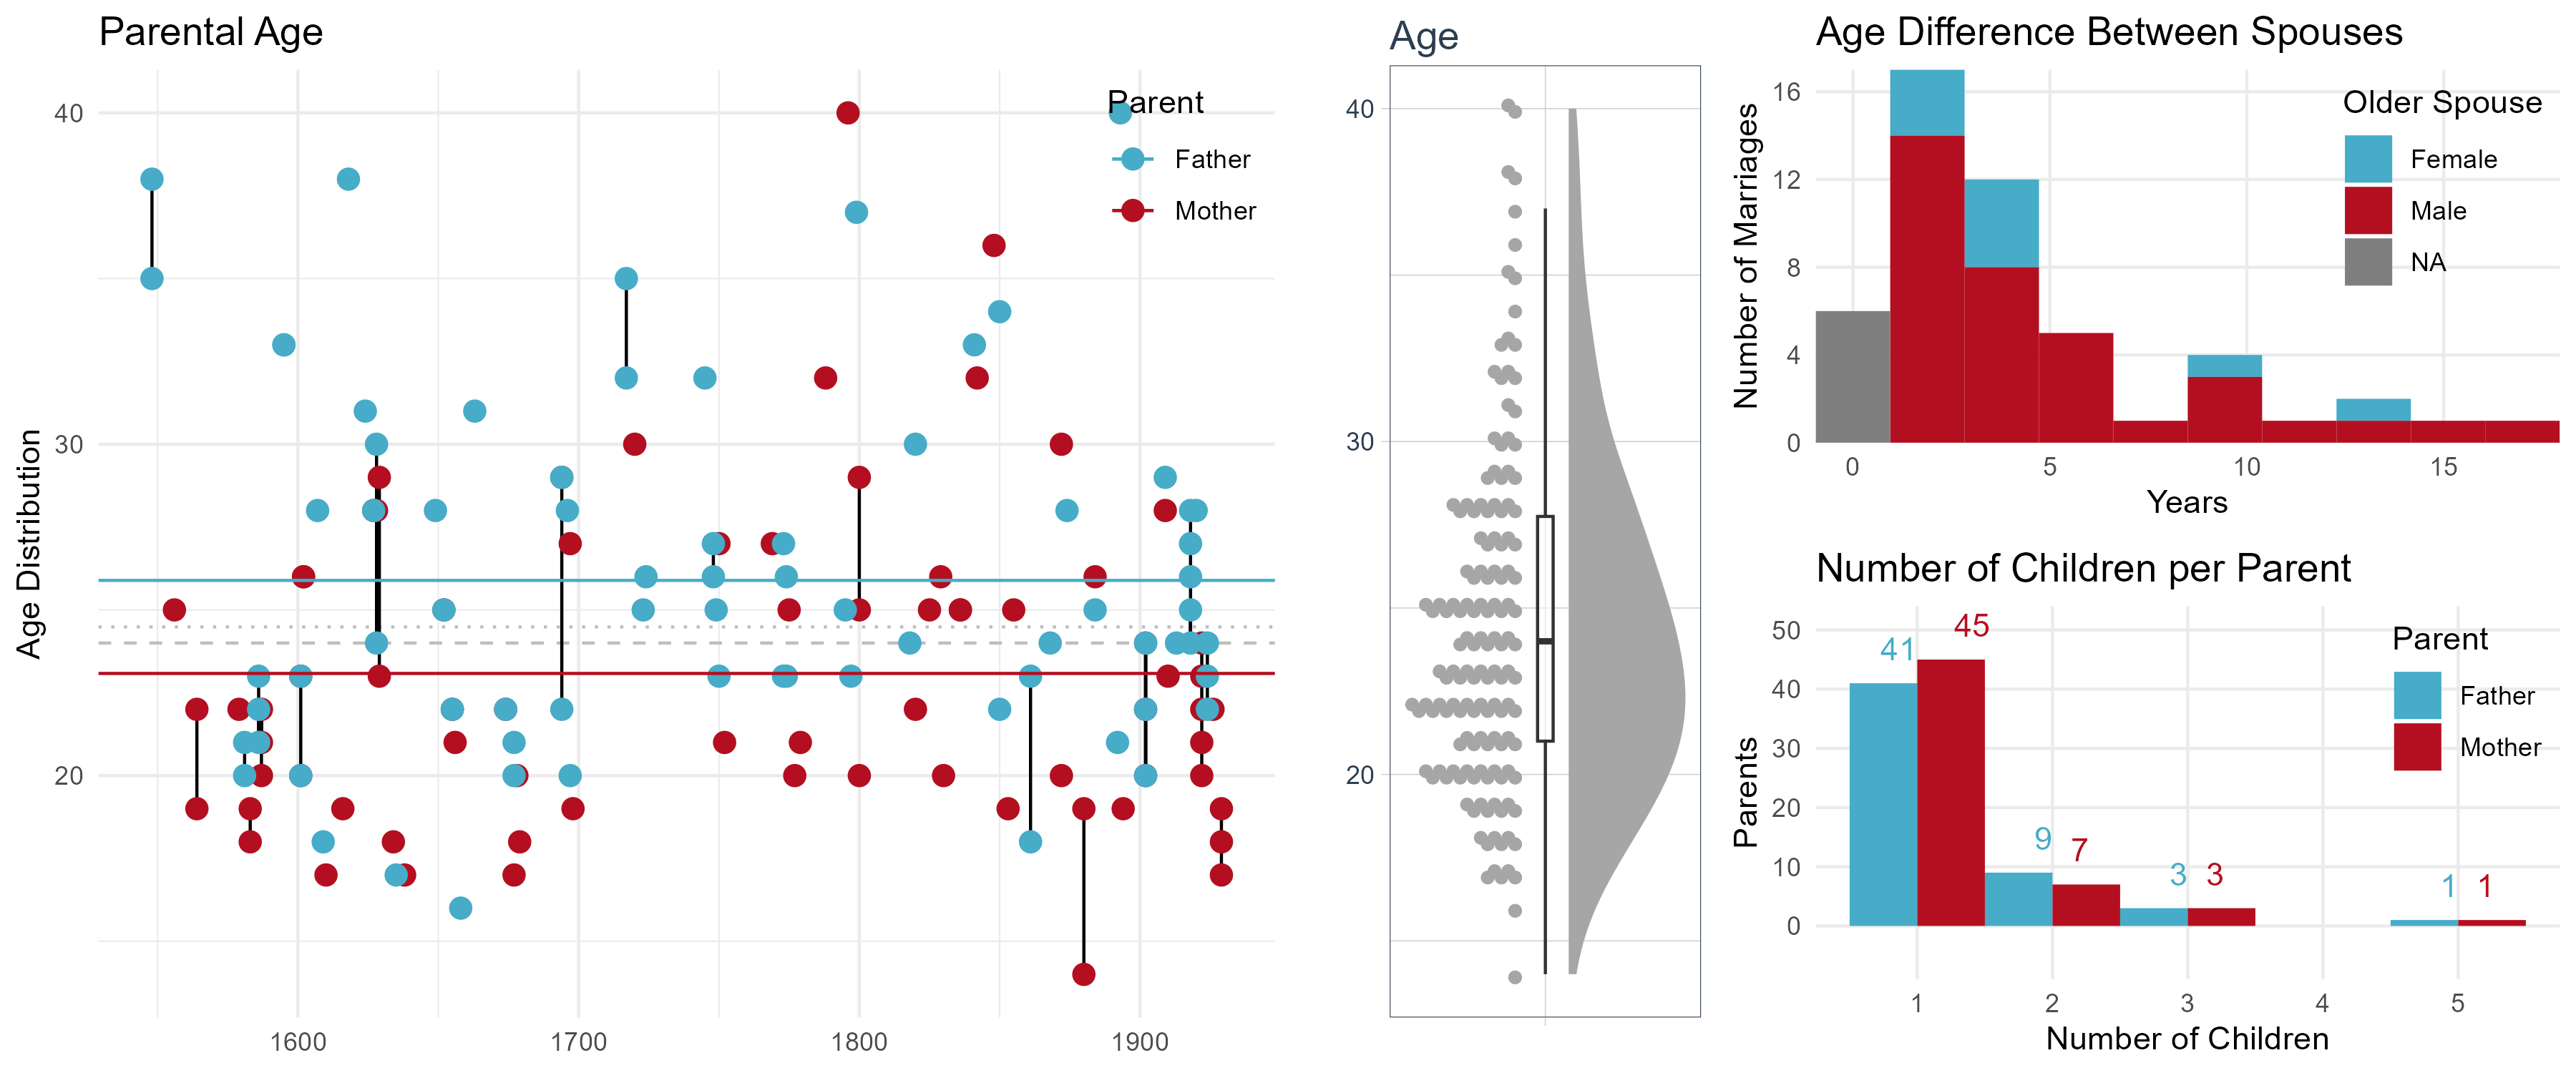
\includegraphics[width=\textwidth]{../rek-data-beers/R/figures/family_parent_age}
    \vspace{-18pt}
    \begin{itemize}
        \item 53 relationships described, 66 children born
        \item 85\% of marriages have an older husband, age difference generally 3 years (max 17 years)
        \item Average age of mother at childbirth is 23.5 years (fathers 26.0)
        \item 22 kids have either no father ($n=10$) or no mother ($n=12$)
    \end{itemize}
\end{frame}
